\subsection{Results}
\newcommand{\cwidth}{.48\linewidth}
\input{../plot/over-one/over-one.tex}

\begin{wrapfigure}[12]{l}{\cwidth}
  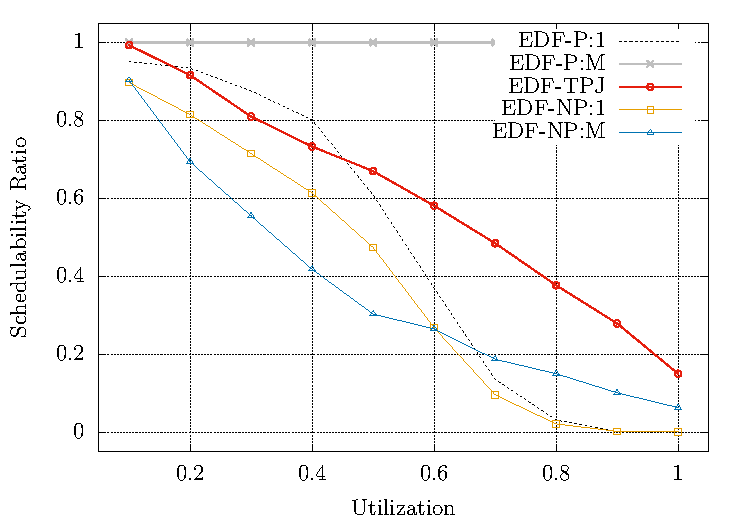
\includegraphics[width=\linewidth]{plot/cs-ratio/cs-ratio}
  \caption{\texttt{BUNDLEP} Case Study}
  \label{fig:cs-ratio}
\end{wrapfigure}

Schedulability ratios from the \bundlep{} case study are given in
Figure~\ref{fig:cs-ratio}. For the target architecture and 18 benchmarks, EDF-TPJ consistently outperforms the other non-preemptive
algorithms. For preemptive EDF-P:1 (with zero cost preemptions), EDF-TPJ
has higher schedulability ratios for the majority of target
utilization values. EDF-TPJ's comparative performance increases
with the target utilization. This case study demonstrates the benefit
of \tpj{} to non-preemptive and (potentially) preemptive approaches.
 
Figures~\ref{fig:avg-ratio-NP-1}, \ref{fig:avg-ratio-NP-m}, and
\ref{fig:avg-ratio-TPJ-i}, summarize the results for the synthetic
task sets varied by the utilization and growth factor. Within
each graph, the schedulability ratios provided by EDF-P:1 and EDF-P:M serve as
references. The difference between EDF-P:1 and the subject of the
graph illustrate the benefit of preemptive scheduling. Inclusion of
EDF-PM highlights the theoretical limit of concave growth to
schedulability.

\begin{wrapfigure}[12]{r}{\cwidth}
  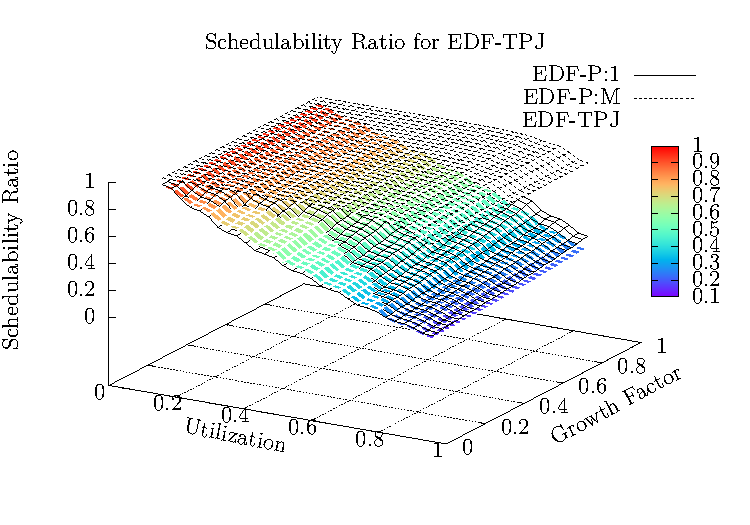
\includegraphics[width=\linewidth]{plot/avg-alg-sched/avg-ratio-TPJ-i}
  \caption{EDF-TPJ Summary}
  \label{fig:avg-ratio-TPJ-i}
\end{wrapfigure}

Including EDF-P:1 and EDF-P:M in each of the summary
graphs eases the comparison between EDF-NP:1, EDF-NP:M, and
EDF-TPJ. Comparing EDF-NP:1 (\ref{fig:avg-ratio-NP-1}) to EDF-NP:M
(\ref{fig:avg-ratio-NP-m}), illustrates the benefits of the model and
scheduling mechanism. EDF-NP:M has a consistently higher
schedulability ratio for all utilizations and growth factors. EDF-TPJ
(\ref{fig:avg-ratio-TPJ-i}) outperforms EDF-NP:M, with higher schedulability
ratios for all utilizations and growth factors due to the ability to
transform task sets. EDF-TPJ performs best among the non-preemptive
tests across all configurations. Additionally, EDF-TPJ is able to
schedule task sets deemed infeasible for EDF-P:1.

\begin{figure}[ht]
  \centering
  \begin{subfigure}{\cwidth}
    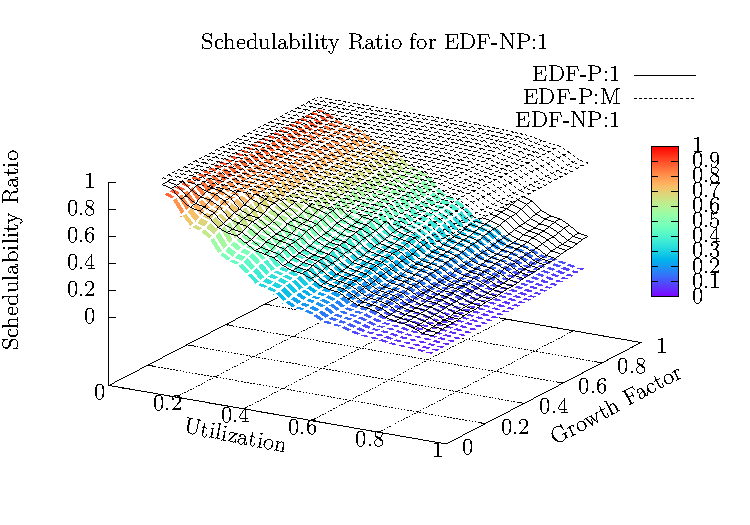
\includegraphics[width=\linewidth]{plot/avg-alg-sched/avg-ratio-NP-1}
    \caption{EDF-NP:1 Summary}
    \label{fig:avg-ratio-NP-1}
  \end{subfigure}%
  \begin{subfigure}{\cwidth}
    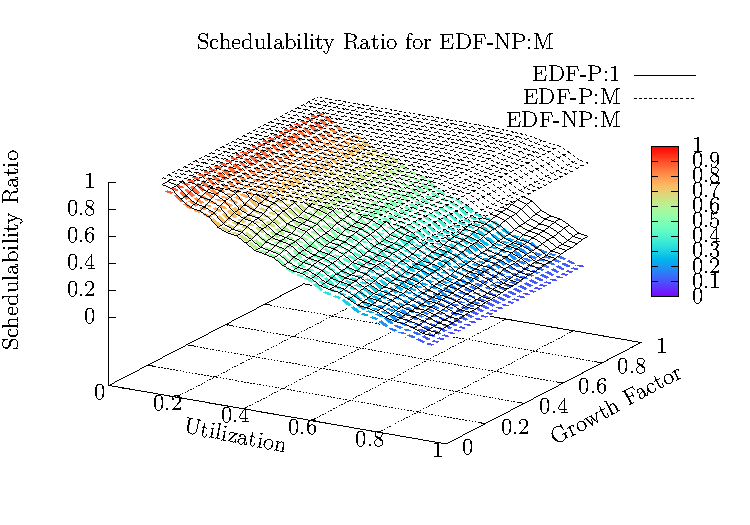
\includegraphics[width=\linewidth]{plot/avg-alg-sched/avg-ratio-NP-m}
    \caption{EDF-NP:M Summary}
  \label{fig:avg-ratio-NP-m}
  \end{subfigure}
  \caption{EDF-NP:1 and EDF-NP:M Summary}
\end{figure}



Table~\ref{table:by-m} summarizes the infeasible utilization
findings for the synthetic tasks. For moderate and larger values of
${M (\ge 25)}$, the number of infeasible by utilization task sets
dominate the specifications. For 25, 50, and 100 total threads, the
infeasible by utilization comprise 44, 59, and 74 percent of the task
sets respectively, with EDF-TPJ finding 25, 34, and 45 percent 
feasible. This illustrates the large potential of the proposed model,
in conjunction with concave growth WCET functions of
thread-level schedulers (e.g. \bundle{} and \bundlep{}).


\begin{wraptable}[11]{r}{.4\linewidth}
  \centering
  \input{../plot/over-one/by-m.tex}
\end{wraptable}

There are two noteworthy trends within the schedulability results.
The simpler of the two is the relationship between utilization and
schedulability ratio for a fixed growth
factor. Figure~\ref{fig:M10F.5} illustrates the trend common among ${M
  \le 10}$ total threads. The trend for preemptive and non-preemptive
schedulability tests when utilization increases is for the
schedulability ratio to decrease. However, EDF-TPJ always outperforms 
the other non-preemptive tests. 

The second trend is slightly more complex. Figure~\ref{fig:M10U.5} was
selected for the smallest ${M}$ and ${U}$ values with visually
distinct plots per schedulability test. The growth factor and the
schedulability ratio are correlated. As the growth factor increases,
so does the schedulability ratio. This is due to the utilization being
held constant. When the growth factor is small, the WCET of the first
thread of each task is larger. Larger WCET values are harder to
schedule non-preemptively.  

\begin{figure}[ht]
  \centering
  \begin{subfigure}{\cwidth}
    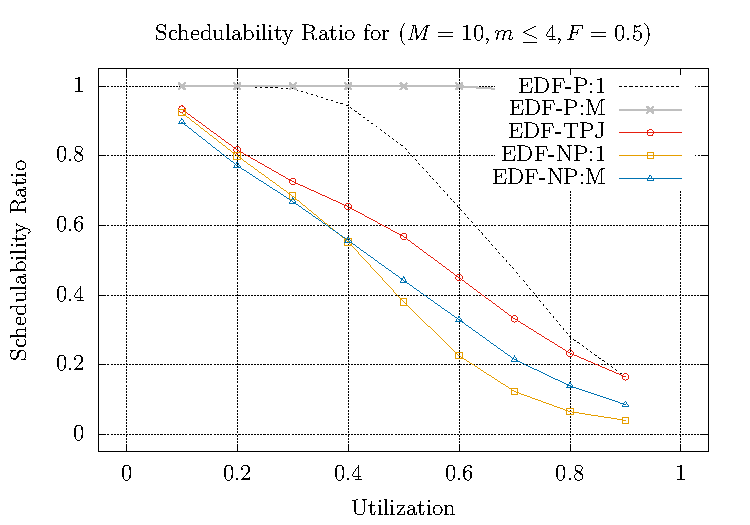
\includegraphics[width=\linewidth]{plot/2D-UFS/2D-M010m04F0_5xS}%
    \caption{${(M,m,U,\GFactor{}) = (10,4,*,0.5)}$}
    \label{fig:M10F.5}
  \end{subfigure}%
  \begin{subfigure}{\cwidth}
    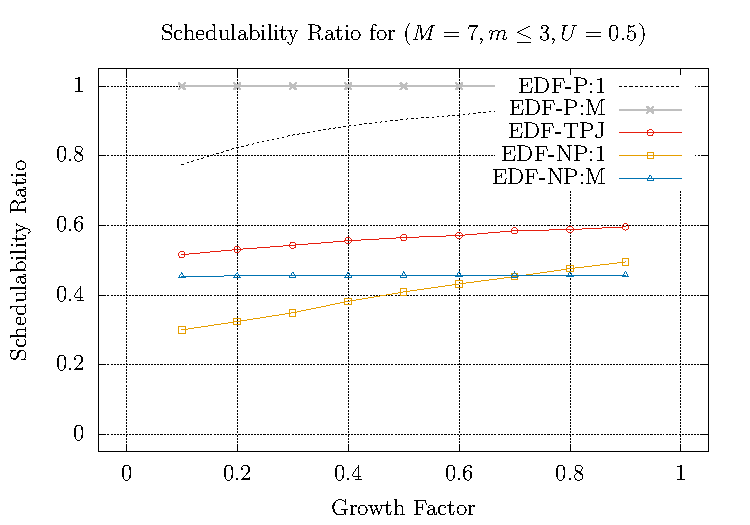
\includegraphics[width=\linewidth]{plot/2D-UFS/2D-M007m03U0_5xS.pdf}%
    \caption{${(M,m,U,\GFactor{}) = (7,3,0.5,*)}$}
    \label{fig:M10U.5}
  \end{subfigure}%
  \caption{${M \le 10}$ Performance}%
\end{figure}

\begin{figure}[ht]
  \centering
  \begin{subfigure}[t]{\cwidth}
    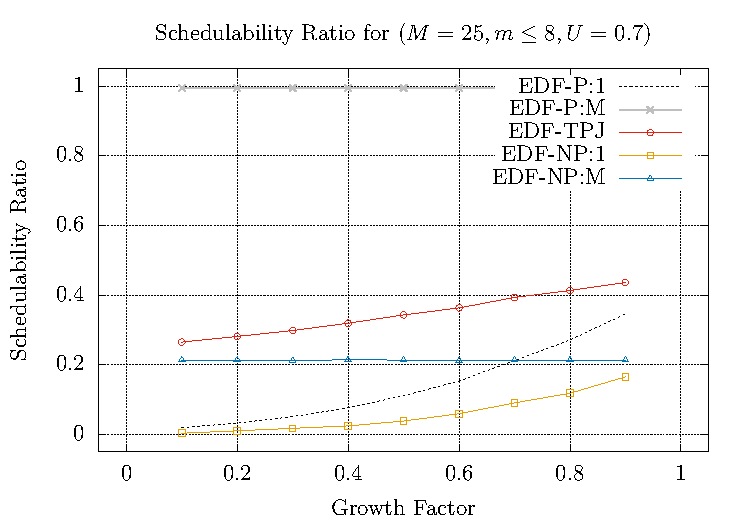
\includegraphics[width=\linewidth]{plot/2D-UFS/2D-M025m08U0_7xS}%
  \end{subfigure}%
  \begin{subfigure}[t]{\cwidth}
    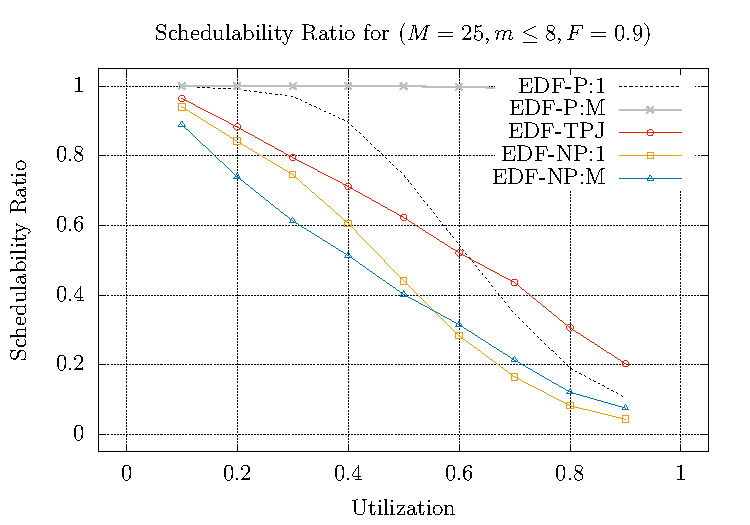
\includegraphics[width=\linewidth]{plot/2D-UFS/2D-M025m08F0_9xS}%
  \end{subfigure}%
  \caption{${M > 10}$ EDF-TPJ Performance Above EDF-P:1}
  \label{fig:m25-tpj}
\end{figure}

As ${M}$ increases beyond 10 total threads, the number of infeasible
by utilization task sets ${s}$ grows. This contributes to the
schedulability ratio of EDF-TPJ surpassing EDF-P:1 for
threshold utilization and growth factor values. For ${M = 25}$, the
threshold of utilization is between ${[0.6,0.7]}$ shown in
Figure~\ref{fig:m25-tpj}.

\begin{figure}[ht]
  \centering
  \begin{subfigure}[t]{\cwidth}
    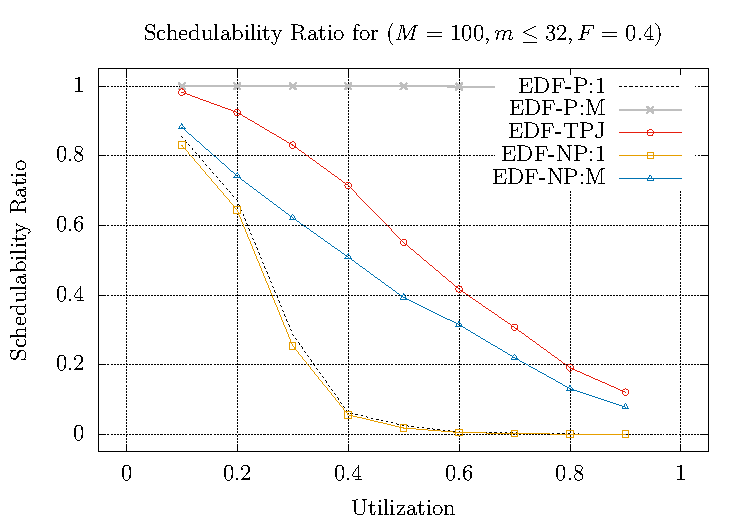
\includegraphics[width=\linewidth]{plot/2D-UFS/2D-M100m32F0_4xS}%
%    \caption{${(M,m,U,\GFactor{}) = (100,32,*,0.4)}$}
  \end{subfigure}%
  \begin{subfigure}[t]{\cwidth}
    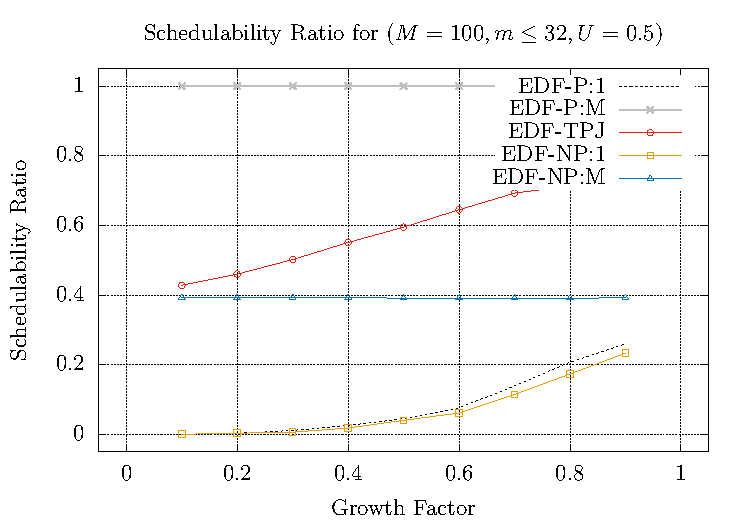
\includegraphics[width=\linewidth]{plot/2D-UFS/2D-M100m32U0_5xS}%
%    \caption{${(M,m,U,\GFactor{}) = (100,32,0.5,*)}$}
  \end{subfigure}%
  \caption{${M = 100}$ EDF-TPJ Performance}
  \label{fig:m100-tpj}
\end{figure}


For ${M = 100}$ and ${\GFactor \le 0.4}$, EDF-TPJ outperforms
EDF-P:1. Figure~\ref{fig:m100-tpj} highlights the advantage of
EDF-TPJ compared to EDF-P:1 by virtue of concave growth. It also
highlights the benefit of dividing tasks, as the performance of
EDF-NP:M is always below EDF-TPJ.


\begin{wrapfigure}[12]{l}{\cwidth}
  \includegraphics[width=\linewidth]{plot/2D-UFS/2D-M003m02U0_7xS}%
  \caption{}
%  \caption{${(M,m,U,\GFactor{}) = (3,2,0.7,*)}$}
  \label{fig:M3U.7}
\end{wrapfigure}

Compared to the non-preemptive tests, EDF-TPJ's performance is
the least beneficial for ${M (< 10)}$ threads and ${U > .4}$
utilization. An example is given in Figure~\ref{fig:M3U.7}, where
EDF-TPJ's schedulability ratio remains below 0.40 for all growth
factors. Preemptive EDF-P:1 schedules nearly double the task sets per
growth factor of EDF-TPJ. This suggests, the decrease in EDF-TPJ's
performance is more likely due to the non-preemptive setting combined
with the larger WCETs of individual threads.
